%%%%%%%%%%%%%%%%%%%%%%%%%%%%%%%%%%%%%%%%%%%%%%%%%%%%%%%%%%%%%%%%%%%%%%%%%%%%%%%%%%%%%%%%%
% Section 6: Placement in RapidSmith2
%	This section contains a description of the following:
%	- How to place cells onto BELs and map cell-pins to bel-pins in RS2
%	- How to get a list of valid placement locations for a cell  
%	- Placement special cases
%%%%%%%%%%%%%%%%%%%%%%%%%%%%%%%%%%%%%%%%%%%%%%%%%%%%%%%%%%%%%%%%%%%%%%%%%%%%%%%%%%%%%%%%%
\newpage
\section{Placement} \label{sec:placement}

In the original RapidSmith, placement occurred at the \cls{Site} level. A
collection of \cls{Cell}s were grouped together in what was called an
\cls{Instance}, and the \cls{Instance} was assigned to a compatible site type.
Where the individual \cls{Cell}s were actually placed within the \cls{Site}
was a blackbox. Because RapidSmith 2 breaks up a \cls{Site} into its
individual components, \cls{Cell}s can now be placed directly onto
physical \cls{BEL}s within a \cls{Site}. This gives Xilinx FPGA CAD developers
finer grain control during the placement of a design, and allows sub-site
algorithms (such as packing algorithms) to be explored. \autoref{code:place}
demonstrates the basic steps to placing a \cls{Cell} in RapidSmith.

\begin{lstlisting} [caption=Steps for placing a Cell in RapidSmith,label=code:place]
// Load the device and design
TincrCheckpoint tcp = VivadoInterface.loadTcp("myCheckpoint.tcp"); 
Device device = tcp.getDevice();
CellDesign design = tcp.getDesign();

// Get a handle to a Cell and Bel. The cell is of type LUT2 
Cell cell = design.getCell("MyCell"); 
Bel bel = device.getSite("SLICE_X40Y137").getBel("D6LUT");

// Place the cell onto the bel
design.placeCell(cell,bel);

// Two ways to map bel pins
CellPin pin1 = cell.getPin("I0");
CellPin pin2 = cell.getPin("I1");
CellPin pin3 = cell.getPin("O")

// First way
pin1.mapToBelPin(bel.getPin("A1"));
pin2.mapToBelPin(bel.getPin("A2"));

// Second way
List<BelPin> possible = pin3.getPossibleBelPins(bel);
pin3.mapToBelPin( possible.get(0) );
\end{lstlisting}

\noindent
As the code listing shows, there are two steps to placing a RapidSmith
\cell. The first is straightforward: get a handle to a \bel object,
and use the method call \texttt{CellDesign.placeCell(Cell, Bel)} (line 11). This
will map a logical \cell onto a physical \bel. Once a \bel has been
used, no other \cells can be mapped to it. No error checking is performed to
ensure that a \cell is compatible with the \bel it is being placed on, that is
up to the user. The second step is more complicated: each logical \cellpin of
the \cell needs to be mapped to a physical \belpin. This can be done by
either (a) specifying the \belpin name (lines 19-20), or (b) using
the function call \texttt{CellPin.getPossibleBelPins(Bel)} (line 23) to
get a list of valid \belpin mappings. For most \cells each \cellpin only
maps to a single \belpin, and so option (b) is preferable. However, there are two
noticable exceptions to this rule.

\begin {enumerate}
  \item LUT input pins are permutable. This means that an input \cellpin 
  attached to a LUT \cell can be mapped to any input pin of a LUT \bel.
  \autoref{fig:lutPins} shows an example of this functionality in Vivado. Once
  the input pins have been mapped, a configuration equation is created for and
  applied to the LUT \bel using the appropriate \belpin inputs.
  In order for a LUT \cell to be physically implemented, these pins need to be
  mapped. The function call \texttt{CellPin.getPossibleBelPins(Bel)} in this
  case will return all of the input \belpins of the LUT and the user can decide
  which ones to use.
  
  \begin{figure}[t]
	\centering
	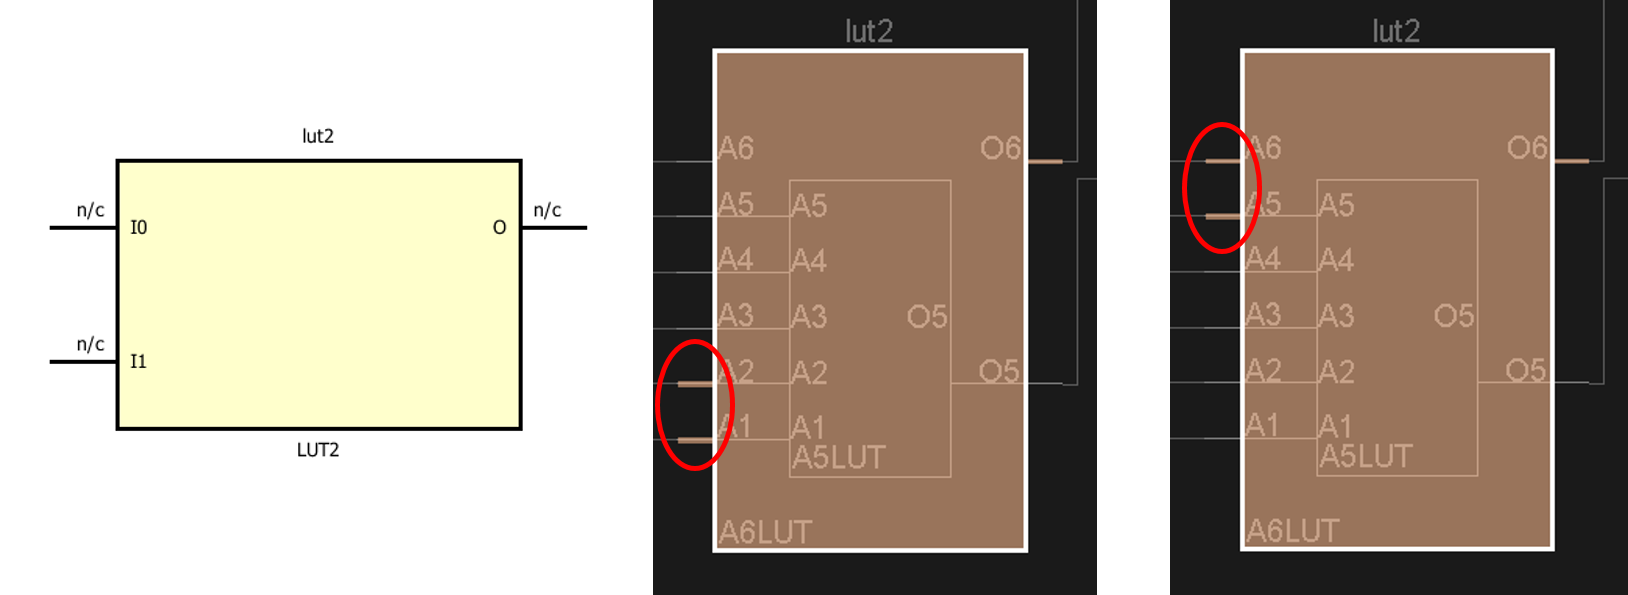
\includegraphics[width=1\columnwidth]{lutPins.png}
	\caption{An example of LUT pin permutations. The left figure shows the
	schematic of a LUT2 cell. The middle figure shows the two input pins of the LUT
	cell being mapped to the A1 and A2 pins of a LUT6 bel. The right figure shows
	the same input pins being mapped to the A6 and A5 pins instead.}
	\label{fig:lutPins}
  \end{figure}
  
  \item Logical-to-physical pin mappings can change \pgm{based on how a cell is
  configured}. For example, on a RAMB36E1 \cell, the least-significant data
  input pins map to different physical \belpins when the width of the BRAM is
  set to 72. This is an important concept when performing netlist modifications
  in RapidSmith. The function call \texttt{CellPin.getPossibleBelPins(Bel)} only
  returns the pin mappings for the \pgm{default} \cell configuration. The
  correct pin mappings are always used when a Tincr checkpoint is imported into
  RapidSmith, but if new logic is being added to a design it is up to the
  user to determine the proper pin mappings. Adding support for
  automatically determining a \cells pin mappings based on a its
  configuration is currently being worked on, but is not yet ready. For now,
  users can configure a cell in Vivado, place it, and use the TCL function shown
  in \autoref{code:tclPinMap} to determine the correct pin mappings for a \cell.

\end{enumerate}

\begin{lstlisting}[language=tcl, caption=TCL script to print all
logical-to-physical pin mappings of a cell,label=code:tclPinMap]

proc print_pin_mappings{cell} {

	foreach cell_pin [get_pins -of $cell] {
		puts "$cell_pin -> [get_bel_pins -of $cell_pin]" 
	}
}

\end{lstlisting}
 
\vspace{.2cm}
\noindent
Some additional points about placement to be aware of include: 

\begin {itemize}
  \item VCC and GND \cells are not placed when implementing a design in Vivado.
  This distinction is applied to RapidSmith 2 as well. Rather than placing VCC
  or GND explictly, \cls{RouteTree}s that are sourced by switchbox TIEOFFs are
  used to express their placement implicitly (VCC/GND is ``placed'' on the
  TIEOFF).
  \item A list of valid placement options for a \cell can be obtained with the
  function call \texttt{Cell.getPossible\-Anchors()}. The sample program
  \pgm{CreateDesignExample} (described in \autoref{sec:createDesignExample})
  gives a good example of how to use this function. The reader is referred to
  the source code and Javadocs for more details.
  \item If you plan on writing a placer in RapidSmith, there are several
  placement rules for a given device. A few examples include (a) CARRY4 \cells
  that are connected through the carry chain need to placed vertically to one
  another so they can use the dedicated carry wires, and (b) A RAMB36E1 cell
  cannot be placed in the same tile as a RAMB18E1 cell. If either of these
  rules are violated, an error will be thrown in Vivado. It is the
  responsibility of the user to determine all relevant placement rules
  because error checking is not performed on design export. The source code for
  a sample simulated annealing placer for the Artix-7 part {\em
  xc7a100tcsg324} can be found in the package
  \pkg{edu.byu.ece.rapidSmith.examples.placerDemo}.
  \item Macro cells in RapidSmith cannot be placed. The internal cells of a
  macro should be placed instead.
\end{itemize}
